%%% PLOT FILE - Responsibility attribution in the winning condition
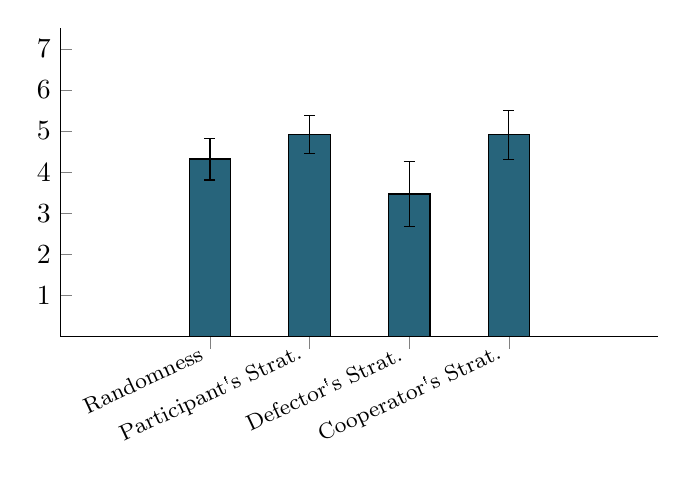
\begin{tikzpicture}%
\begin{axis}[%
    ybar,
    %title=Test,%
    axis y line*=left, axis x line*=bottom,%
    ymin=0,
    ymax=7.5,
    ytick={1,2,...,7},
    %legend style={at={(1.4,1)}},
    x tick label style={rotate=25,anchor=east},
    symbolic x coords={Randomness,Participant\textquotesingle s Strat.,Defector\textquotesingle s Strat.,Cooperator\textquotesingle s Strat.},%
    xtick=data,
    x=36pt,
    enlarge x limits=0.5,
    height=5.5cm,
    bar width=15pt,
    xticklabel style={font=\footnotesize},]%
\addplot+[
    color=black,
    fill={rgb,255:red,39; green,100; blue,123},%
    %postaction={pattern= north east lines},
    error bars, y dir=both, y explicit]
				coordinates {
				(Randomness,4.32) +- (Randomness,0.51)
				(Participant\textquotesingle s Strat.,4.91) +- (Participant\textquotesingle s Strat.,0.46)
				(Defector\textquotesingle s Strat.,3.47) +- (Defector\textquotesingle s Strat.,0.78)
				(Cooperator\textquotesingle s Strat.,4.91) +- (Cooperator\textquotesingle s Strat.,0.6)};
%\legend{Winning,Losing}
\end{axis}%
\end{tikzpicture}%